% -*- mode: LaTeX; TeX-PDF-mode: t; -*-  # Config emacs auctex

% allow latex to find custom stuff
% Add the listed directories to the search path
% (allows easy moving of files around later)
% these paths are searched AFTER local config kpsewhich

% *.sty, *.cls
\makeatletter
\def\input@path{{@resources/texlive/texmf-local/tex/latex//}
        ,{@resources/texlive/latex//}
        ,{@local//}
        }
\makeatother
\makeatletter
\def\bibinput@path{{@resources/texlive/texmf-local/tex/latex//}
        ,{@resources/texlive/latex//},
        ,{@local//}
        }
\makeatother
  

% Set paths (like, \LaTeXInputs) to find resources
\newcommand{\econtexRoot}{.}
 

\documentclass[pdflatex,aspectratio=169]{beamer}

\usepackage{pdfsuppressruntime}

\usepackage{multirow}

\newbool{fullcon}\global\booltrue{fullcon}\boolfalse{fullcon} %full content, 30-40 min
\newbool{bundesb}\global\booltrue{bundesb}\boolfalse{bundesb} %reduced, 20 min presentation
\newbool{upenn}\global\booltrue{upenn}%\boolfalse{upenn} %reduced, 20 min presentation
\usepackage{econark}


% _____________ Opening slide _______________________


\title[Stimulus]{Welfare and Spending Effects of Consumption Stimulus Policies}
\author{
  Christopher D.\ Carroll (JHU)
  \and
  Edmund Crawley (FED)
  \and
  William Du (JHU)
  \and
  Ivan Frankovic (BBK)
  \and
  H{\aa}kon Tretvoll (SSB)
}

\ifbool{upenn}{\date[\today]{University of Pennsylvania, 2024-11-06  \\ \medskip \medskip \medskip \href{https://econ-ark.org/}{\small Powered By} \\ 
\includegraphics[width=0.5in]{./@resources/econ-ark/econ-ark-logo-small.png}}}

\ifbool{bundesb}{
      \date[\today]{CEF - July 6, 2023  \\ \medskip \medskip \medskip
        \href{https://econ-ark.org/}{\small Powered By} \\ 
\includegraphics[width=0.5in]{econ-ark-logo-small.png}}}{}
    
\ifbool{fullcon}{
    \date[\today]{SSB Fiscal Policy Workshop - May 25, 2023  \\ \medskip \medskip \medskip 
          \href{https://econ-ark.org/}{\small Powered By} \\ 
\includegraphics[width=0.5in]{econ-ark-logo-small.png}}}{}

\newcommand{\RNum}[1]{\uppercase\expandafter{\romannumeral #1\relax}}

\AtBeginSection[]{
  \begin{frame}
    \vfill
    \centering
    \begin{beamercolorbox}[sep=8pt,center,shadow=true,rounded=true]{title}
      \usebeamerfont{title}\insertsectionhead\par%
    \end{beamercolorbox}
    \vfill
  \end{frame}
}

\usepackage[font=small,skip=0pt]{caption}
\usepackage{booktabs}

\usepackage{comment}

\renewcommand{\PermGroFac}{G}

\begin{document}\bibliographystyle{econark}

\begin{frame}[plain]
  \titlepage
  
  \footnotesize{Viewpoints and conclusions stated in this paper are the responsibility of the authors alone
    and do not necessarily reflect the viewpoints of The Federal Reserve Board or The Deutsche Bundesbank.}
\end{frame}


% _____________ 1st section  ____________


\begin{frame}
  \frametitle{Motivation}
  \begin{itemize}[<+->]
  \item Fiscal policies to boost $C$ in recessions
    \begin{itemize}[<+->]
    \item many different policies tried in many countries in recent decades  
    \end{itemize}
  \item Why so much variation in policies?

    \begin{itemize}[<+->]
      \itemsep = .25\bigskipamount 
    \item no guidance from traditional RANK models	
      \begin{itemize}[<+->]
      \item tiny MPC's: $C$ stimulus ineffective
      \item away from ZLB, monetary policy should work
      \end{itemize}
    \item also likely variation in objectives:
      \begin{itemize}[<+->]
      \item increase output (`GDP metric')
      \item reduce misery (`welfare metric')
      \end{itemize}
    \end{itemize}
    \bigskip
    \pause
  \textbf{What Do We Do?}
  \begin{itemize}[<+->]
    \item Comparative effectiveness of three policies
    \begin{itemize}[<+->]
      \item Stimulus checks
      \item Extended UI
      \item Payroll tax cuts
      \end{itemize}
  \end{itemize}
\end{itemize}
\end{frame}


\begin{frame}
  \frametitle{Related literature}
  \small
  \begin{itemize}[<+->]
  \item \textbf{Effects of transitory income shocks}: 
    Parker, Souleles, Johnson and McClelland (2013); Broda and Parker (2014); Fagereng, Holm and Natvik (2021); Ganong, Greig, Noel, Sullivan and Vavra (2022)
  \item \textbf{HA models consistent with high MPCs}: 
    Kaplan and Violante (2014); Auclert, Rognlie and Straub (2018); Carroll, Crawley, Slacalek and White (2020); Kaplan and Violante (2022) 
  \item \textbf{State dependent multipliers (ZLB)}: 
    Christiano, Eichenbaum and Rebelo (2011); Eggertson (2011); Ramey and Zubairy (2018); Hagedorn, Manovskii and Mitman (2019) 
  \item \textbf{Extended unemployment insurance}:
    Ganong, Greig, Noel, Sullivan and Vavra (2022); Kekre (2022) 
  \item \textbf{Welfare measures in HA models}:
    Bhandari, Evans, Golosov and Sargent (2021); D{\'a}vila and Schaab (2022)
    % \item \textbf{High MPCs and impatience}: Parker (2017)
  \end{itemize}
  \normalsize
\end{frame}

\begin{frame}
  \frametitle{Quantitative Economics}
  \begin{itemize}[<+->]
    \item These are \textit{quantitative} questions: require \textit{quantitative} realism ...
    \item ... about the differences that make a difference
    \begin{itemize}[<+->]
    \item UI
      \begin{itemize}[<+->]
      \item Is not Calvo!
        \item Makes a big difference quantitatively
      \end{itemize}
    \item Distributions of income, wealth
      \begin{itemize}
      \item Profoundly important for (i)MPCs
      \end{itemize} 
      \item Differences in unemployment risks
      \item Heterogeneity in income growth rates
  \end{itemize}
\end{itemize}

\pause Treatment of Multiplier?

\begin{itemize}[<+->]
  \item Baseline is NOT a HANK model:
    \begin{itemize}[<+->]
    \item HANK Mechanisms behind multipliers are v. complex
    \item Away from ZLB, multipliers not necessarily much different in recessions
    \item Far from clear if timing is right
    \end{itemize}
  \end{itemize}
  
  \begin{itemize}[<+->]
    \itemsep = .25\bigskipamount 
    \item Robustness Exercise: HANK model 
    \end{itemize}
\end{frame}

\begin{frame}
  \frametitle{Quantitative Micro Realism}

  Idiosyncratic income process: Friedman/Muth (transitory and permanent shocks)
  \providecommand{\permLvl}{}\renewcommand{\permLvl}{\permLvlInd}
  \begin{eqnarray}
    \permLvlInd & - & \text{`permanent income'} \\
\tranShkInd & - & \text{`transitory income shock'}  \\
    \permShk & - & \text{`permanent income shock'}
  \end{eqnarray}
  \begin{equation}\begin{gathered}\begin{aligned}
    \permLvlInd_{t+1} & = \PermGroFac \permLvlInd_{t} \permShk_{t+1} \\
    y_{t+1} &= \permLvlInd_{t+1}\tranShkInd_{t+1} \\
  \end{aligned}\end{gathered}\end{equation}
\end{frame}

\begin{frame}\frametitle{Evidence?}
  \providecommand{\var}{}\renewcommand{\var}{\mathrm{var}}
  For $n>3$,
  \begin{equation}
    \var(\log y_{t+n}/y_{t}) = 2 \sigma^{2}_{\log \tranShkInd} + n \sigma^{2}_{\log \permShkInd}
  \end{equation}
  Millions of datapoints from Norwegian National Registry:
  \begin{center}
    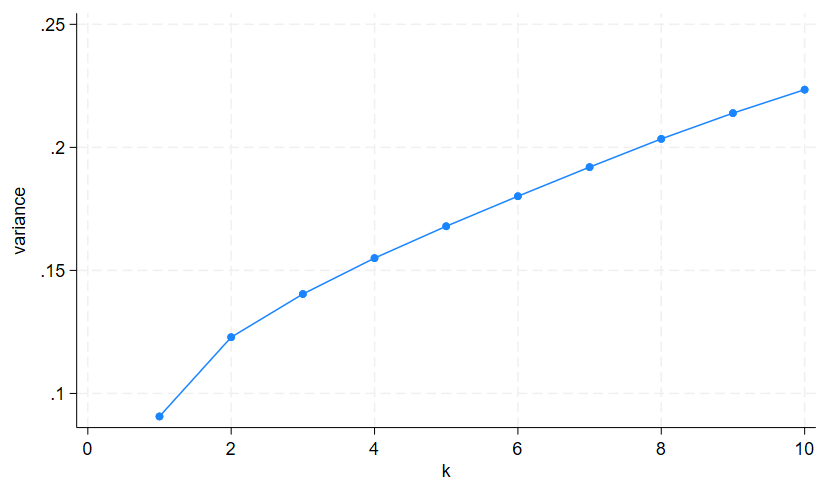
\includegraphics[width=0.5\linewidth]{./Figures/norway_income_change_variance.png}

    Source: SSB (Elin Halvorsen)
  \end{center}
  Also see Crawley, Holm, and Tretvoli (2022)
\end{frame}

\begin{frame}
  \frametitle{Preferences, Beliefs, and Wealth}
  Infinite horizon model: target wealth depends on `Growth Impatience' condition:
\begin{equation}
  \underbrace{
    \left(
      \frac{(\Rfree \DiscFac)^{1/\gamma}}
      {\PermGroFac\Ex[\permShk^{-1}]}
    \right)
    }_{\text{'Growth Patience Factor'}}
      < 1
    \end{equation}
    
  \pause 
  \emph{Degree} of impatience (1-GPF) determines \emph{size} of target
  \begin{itemize}[<+->]
  \item If GPF $\geq 1$, target is $\infty$
    \item if everybody has same GPF, target wealth is identical
    \item Fact: Wealth much more unevenly distributed than permanent income
      \item $\Rightarrow$ need heterogeneity in GPF
  \end{itemize}

  \hypertarget{ConsistentWithMicroData}{}

  \pause
  We use
  \begin{itemize}[<+->]
  \item \textit{Ex-ante} heterogeneity in discount factors
  \item $\PermGroFac$ or $\Rfree$ would do as well
  \end{itemize}
  
\end{frame}

\begin{frame}
  \frametitle{Consistency With Micro Evidence?}
  \begin{columns}
    \begin{column}{0.5\textwidth}
      Liquid Wealth from \href{https://www.federalreserve.gov/econres/scfindex.htm}{SCF}
      
      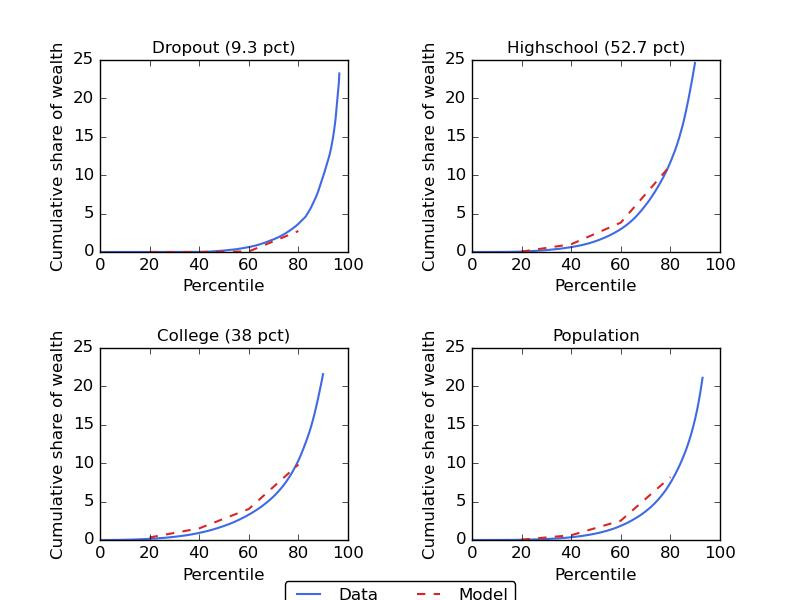
\includegraphics[width=\linewidth]{\FigDir/LorenzPoints}
      
    \end{column}
    
    \pause
    
    \begin{column}{0.4\textwidth}  	
      Intertemporal MPC from Fagereng, Holm, Natvik (2021)	
      
      \includegraphics[width=\linewidth]{\econtexRoot/Code/HA-Models/Target_AggMPCX_LiquWealth/Figures/AggMPC_LotteryWin}
      
      Modeling device: `Splurge' in consumption, i.e. exogenously given fraction of income directly consumed
    \end{column}
  \end{columns}
  
\end{frame}



    \begin{frame}
      \frametitle{Evaluation of consumption stimulus policies in the US}
      \begin{itemize}[<+->]
        \itemsep = .5\bigskipamount 
      \item Policies we consider: 
        \begin{itemize}[<+->]
          \itemsep = .25\bigskipamount 
        \item Stimulus check for \$1200 (means-tested)
        \item Extension of unemployment benefits from 6 months to 1 year
        \item Payroll tax cut by 2\% for 2 years
        \end{itemize}
        % \item Key features of the policies: 
        %   \begin{itemize}[<+->]
        %     \itemsep = .25\bigskipamount 
        %   \item Targeting 
        %   \item Timing of spending (overlap with recession!)
        %   \item Scalability 
        %   \end{itemize}
        \bigskip
      \item Evaluation criteria: 
        \begin{itemize}[<+->]
          \itemsep = .25\bigskipamount 
        \item Spending multipliers
        \item Welfare (only recession-related welfare impact)
        \end{itemize}
      \end{itemize}
    \end{frame}


    \begin{frame}
      \frametitle{Preview of results}
      \begin{itemize}[<+->]
        \itemsep = \bigskipamount 
      \item Welfare measure: Extension of UI benefits is the clear winner 
        \begin{itemize}[<+->]
          \itemsep = .25\bigskipamount 
        \item Targeted at individuals with high MPCs and high recession-related welfare losses
        \item But: higher spending may continue after recession is over 
        \end{itemize}
      \item Spending multiplier: Stimulus check has the highest multiplier 
        \begin{itemize}[<+->]
          \itemsep = .25\bigskipamount 
        \item Not well targeted, but increases income immediately 
          % \item Also: easy to scale up
        \end{itemize}
      \item Tax cut
        \begin{itemize}[<+->]
          \itemsep = .25\bigskipamount 
        \item Poorly targeted and much spending likely to occur after end of recession
        \end{itemize}
      \end{itemize}
    \end{frame}






    \section{Model}

    \begin{frame}
      \frametitle{Consumer problem}


      \begin{itemize}[<+->]
      \item Education groups: "Dropout", "Highschool" and "College"
      \item Each group has distribution of discount factors $\beta_i$
      \item Idiosyncratic, stochastic income process $\mathbf{y}_{i,t}$
      \item Estimated splurge factor $\varsigma$: $\mathbf{c}_{sp,i,t} = \varsigma \mathbf{y}_{i,t}$
        \pause
      \item Remaining consumption $c_{opt,i,t}$ is chosen to maximize utility
        \begin{equation}\begin{gathered}\begin{aligned}
          \sum_{t=0}^{\infty}\beta_i^t (1-D)^t \mathbb{E}_0 u(\mathbf{c}_{opt,i,t}).
        \end{aligned}\end{gathered}\end{equation}
        ($D$: end-of-life probability, $u$: stand.
CRRA utility func.)	
      \item Budget constraint, given existing market resources $m_{i,t}$ and income state, and a no-borrowing constraint: 
        \begin{equation}\begin{gathered}\begin{aligned}
          \mathbf{m}_{i,t+1} &= R \underbrace{(\mathbf{m}_{i,t} - \mathbf{c}_{sp,i,t} - \mathbf{c}_{opt,i,t})}_{\geq 0 \text{ (no-borrowing constraint)}} + \mathbf{y}_{i,t+1}
        \end{aligned}\end{gathered}\end{equation}
        ($R$: exogenous gross interest rate)
      \end{itemize}



    \end{frame}


    \begin{frame}
      \frametitle{ Income process}

      \begin{itemize}[<+->]

      \item Income subject to transitory, unempl. and permanent shocks
        \begin{equation}\begin{gathered}\begin{aligned}
          \mathbf{y}_{i,t} =   \begin{cases}
            \xi_{i,t}\mathbf{p}_{i,t}, & \text{if employed} \\
            0.7 \mathbf{p}_{i,t}, & \text{if unemployed for $\leq$ 2q} \\
            0.5 \mathbf{p}_{i,t}, & \text{if unemployed $\ge$ 2q} 
          \end{cases}
        \end{aligned}\end{gathered}\end{equation}
        ($\xi_{i,t}$: trans.
shock, $p$: perm.
income)
        
      \item "Permanent income":  $\mathbf{p}_{i,t+1} = \underbrace{\psi_{i,t+1}}_{\text{perm.
shock}} \underbrace{\Gamma_{e(i)}}_{\text{educ.-specific growth}}\mathbf{p}_{i,t}$ 


        \pause
        \bigskip
      \item Employment status is subject to a Markov process
        \begin{itemize}[<+->]
        \item Unemployment rate education-specific (doubles in recession)
        \item Expected length of unemployment: 1.5q  (4q in recession)
        \end{itemize}
        
      \item Recession is given by an MIT shock; end of recession as a Bernoulli process (avg.
length of 6q)
        
        
      \end{itemize}

    \end{frame}






    % \ifbool{fullcon}{	
    %   \begin{frame}
    %     \frametitle{Three policies to fight the recession - Details}
    %     
    %     \begin{itemize}[<+->]
    %     \item Stimulus check
    %       \begin{itemize}[<+->]
    %       \item Everyone receives a check for \$1,200 in q1 of the recession
    %       \item Check is means-tested: Full check if perm. income $\leq$ \$100k; Falls linearly for higher incomes and zero for those $\geq$ \$150k
    %       \end{itemize}
    %       
    %     \item Extended unemployment benefits
    %       \begin{itemize}[<+->]
    %       \item Unemployment benefits are extended from 2 to 4 q
    %       \item Extension occurs regardless of whether recession ends
    %       \end{itemize}
    %       
    %     \item Payroll tax cut
    %       \begin{itemize}[<+->]
    %       \item Employees payroll tax rate is reduced such that income rises by 2\% for 8q	
    %       \end{itemize}
    %     \end{itemize}
    %     
    %     Policies are debt-financed and repayed much later
    %   \end{frame}
    % }{}

    \begin{frame}
      \frametitle{Aggregate demand effects \\ 
        \small (as in Krueger, Mitman and Perri, 2016) \normalsize}
      \begin{itemize}[<+->]
        \itemsep = .5\bigskipamount 
      \item Baseline: No feedback from aggregate consumption to income
      \item Extension: We allow for aggregate demand effects from consumption on income during the recession
        
      \item The AD effect is given by
        \begin{equation}\begin{gathered}\begin{aligned}
          AD(C_t) =   \begin{cases}
            \Big(\frac{C_t}{\tilde{C}}\Big)^\kappa, & \text{if in a recession} \\
            1, & \text{otherwise} ,
          \end{cases}
        \end{aligned}\end{gathered}\end{equation}
        where $\tilde{C}$ is the level of consumption in the steady state.

        
      \item Idiosyncratic income in the extension model is then given by
        \begin{equation}\begin{gathered}\begin{aligned}
          \mathbf{y}_{AD,i,t} = AD(C_t)\mathbf{y}_{i,t}.
        \end{aligned}\end{gathered}\end{equation}
      \end{itemize}
    \end{frame}



    \ifbool{fullcon}{

        \section{Parametrization}

        \begin{frame}
          \frametitle{Parametrization --- Strategy}
          \begin{itemize}[<+->] 
            \itemsep = \bigskipamount 
          \item Step 1: Estimate the splurge factor in a Norwegian version of the economy --- match iMPCs from FHN (2021)
          \item Step 2a: Calibrate a set of parameters that affect all education groups equally 
          \item Step 2b: Calibrate a set of parameters that match features of the different education groups 
          \item Step 3: Estimate a discount factor distribution for each education group to match within-group distribution of liquid wealth
            \begin{itemize}[<+->]
              \itemsep = .25\bigskipamount 
            \item $\beta_e$: center of discount factor distribution
            \item $\nabla_e$: spread of discount factor distribution 
            \item Uniform distribution, approximated with 7 different types
            \end{itemize}
          \end{itemize} 
        \end{frame}

        \begin{frame}
          \frametitle{Step 1: iMPC from FHN (2021)}
          \centering 
          %	\includegraphics[width=3in]{\FigDir/AggMPC_LotteryWin}
          \includegraphics[width=3in]{\econtexRoot/Code/HA-Models/Target_AggMPCX_LiquWealth/Figures/AggMPC_LotteryWin}
          \begin{itemize}[<+->]
            \itemsep = .5\bigskipamount 
          \item Estimated splurge factor: $\varsigma = 0.31$; MPC across wealth distrubtion and K/Y untargeted but close to targets
          \item Zero splurge ($\varsigma = 0$): cannot match iMPC, wealth-dep. MPCs and K/Y-ratio at the same time
          \end{itemize}
        \end{frame}

        \begin{frame}
          \frametitle{Step 2a: Parameters --- same for all types  \hyperlink{sli:policies}{\beamerbutton{Policy parameters}} }
          \hypertarget{Parameters}{}
          \begin{tabular}{lcd{3}} 
            \toprule
            \multicolumn{3}{l}{Parameters that apply to all types} \\ \midrule	
            Parameter & Notation & \text{Value} \\ \midrule 
            Risk aversion & $\gamma$ & 2.0 \\ 
            Splurge & $\varsigma$ & 0.306 \\ 
            Survival probability, quarterly & $1-D$ & 0.994 \\
            Risk free interest rate, quarterly (gross) & $R$ & 1.01 \\ 
            Standard deviation of transitory shock & $\sigma_\xi$ & 0.346 \\
            Standard deviation of permanent shock & $\sigma_\psi$ & 0.0548 \\ 
            Unemployment benefits replacement rate (share of PI) & \textcolor{red}{$\rho_b$} & \textcolor{red}{0}.\textcolor{red}{7} \\ 
            Unemployment income w/o benefits (share of PI) & \textcolor{red}{$\rho_{nb}$} & \textcolor{red}{0}.\textcolor{red}{5} \\ 
            Avg. duration of unemp. benefits in normal times (quarters) & & 2 \\
            Avg. duration of unemp. spell in normal times (quarters) & & 1.5 \\
            Probability of leaving unemployment & $\pi_{ue}$ & 0.667 \\ 
            Consumption elasticity of aggregate demand effect & $\kappa$ & 0.3 
            \\ \bottomrule 
          \end{tabular}
        \end{frame}


        \begin{frame}
          \frametitle{Step 2b: Parameters --- by education group}
          \label{sli:paramsByEd}
          \begin{tabular}{lccc}
            \toprule 
            \multicolumn{4}{l}{Parameters calibrated for each education group} \\ \midrule
            & Dropout & Highschool & College \\ \midrule
            Percent of population & \phantom{0}9.3 & 52.7 & 38.0 \\ 
            Avg. quarterly PI of ``newborn'' agent (\$1000) & \phantom{0}6.2 & 11.1 & 14.5 \\
            Std. dev. of $\log($PI$)$ of ``newborn'' agent & 0.32 & 0.42 & 0.53 \\
            Avg. quarterly gross growth rate of PI ($\Gamma_e$) & 1.0036 & 1.0045 & 1.0049 \\
            Unemployment rate in normal times (percent) & \phantom{0}8.5 & \phantom{0}4.4 & \phantom{0}2.7 \\ 
            Probability of entering unemployment ($\pi_{eu}^{e}$, percent) & \phantom{0}6.2 & \phantom{0}3.1 & \phantom{0}1.8 
            \\ \bottomrule 
          \end{tabular}
        \end{frame}


        \begin{frame}
          \frametitle{Step 3: Estimation of discount factors}
          \begin{tabular}{lccc}
            & Dropout & Highschool & College \\ \midrule
            $(\beta_e, \nabla_e)$ & (0.735, 0.298) & (0.924, 0.137) & (0.984,0.010) \\
            (Min, max) in approximation & (0.480, 0.991) & (0.806, $0.989^*$) & (0.976, 0.992) \\
            \midrule 
          \end{tabular} 
          \begin{tabular}{lccc}
            \multicolumn{4}{l}{ } \\ \midrule
            \textbf{Estimation targets} & Dropout & Highschool & College \\ \midrule
            Median LW/ quarterly PI (data, percent) & 4.64 & 30.2 & 112.8 \\ 
            Median LW/ quarterly PI (model, percent) & 4.64 & 30.2 & 112.8 %\\
            % $[20,40,60,80]$ pctiles of Lorenz curve (data) & $[0, 0.01, 0.6, 3.6]$ & $[0.06, 0.6, 3.0, 11.6]$ & $[0.2, 0.9, 3.3, 10.3]$ \\
            % $[20,40,60,80]$ pctiles of Lorenz curve (model) & $[0.0, 0.0, 0.5, 3.6]$ & $[0.04, 0.9, 3.7, 11.3]$ & $[0.3, 1.5, 4.0, \phantom{0}9.9]$
            \\ \midrule 
          \end{tabular} 
          \begin{tabular}{lcccc}
            \multicolumn{5}{l}{ } \\ \midrule
            \textbf{Non-targeted moments} & Dropout & Highschool & College & Population \\ \midrule
            Percent of total wealth (data) & 0.8 & 17.9 & 81.2 & 100 \\
            Percent of total wealth (model) & 1.1 & 21.9 & 77.0 & 100 \\
            Avg. annual MPC (model, incl. splurge) & 0.87 & 0.71 & 0.48 & 0.64
            \\ \bottomrule 
          \end{tabular}
        \end{frame}




        \begin{frame}
          \frametitle{Step 3: Visualization of match with SCF}
          \centering
          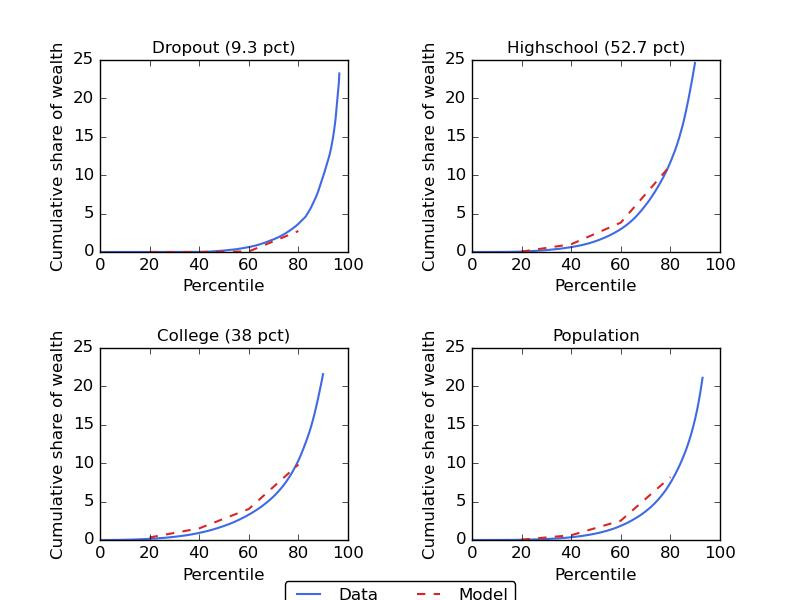
\includegraphics[width=4in]{\FigDir/LorenzPoints}
        \end{frame}


      }{}

      \section{Results}


      \ifbool{bundesb}{

          \begin{frame}
            \frametitle{Impulse responses}


            \begin{columns}	
              
              
              \begin{column}{0.5\textwidth} 
                \small 	
                \begin{itemize}[<+->]
                \item Simulate policies in recessions lasting 1 to 20 q
                \item Construct probability-weighted sum across rec. lengths
                \end{itemize}
              \end{column}	
              
              
              \begin{column}{0.4\textwidth}  
                \footnotesize Stimulus check:
                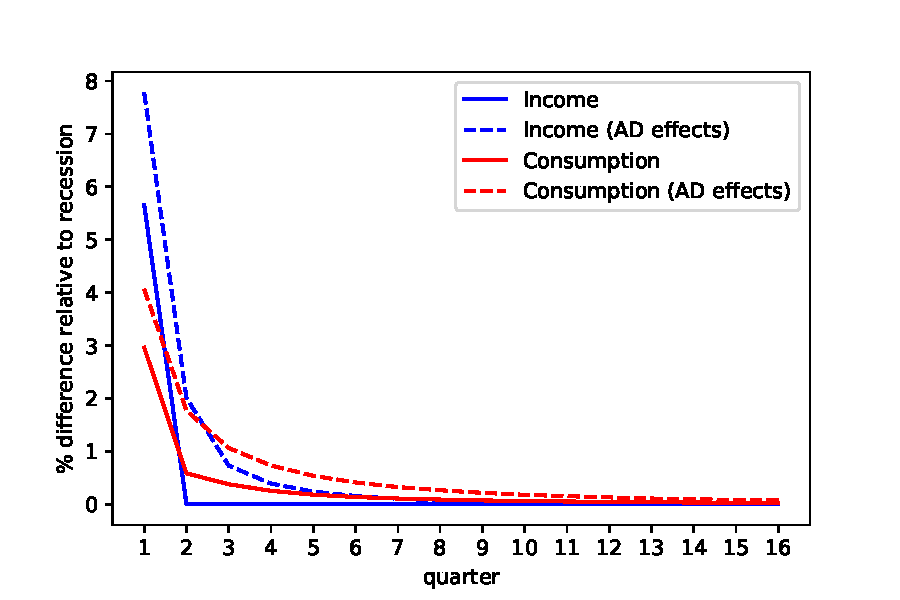
\includegraphics[width=\linewidth]{\econtexRoot/Code/HA-Models/FromPandemicCode/Figures/recession_Check_relrecession}
                
              \end{column}  	

            \end{columns}

            \pause
            
            \begin{columns}	
              
              \begin{column}{0.33\textwidth}  	
                \footnotesize Extension of UI benefits:
                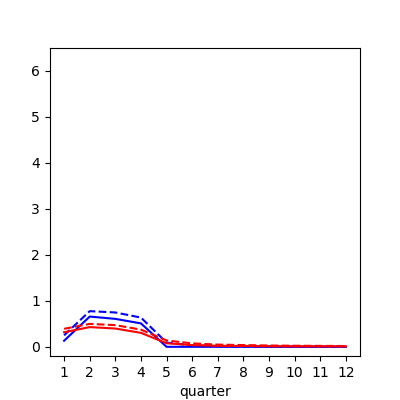
\includegraphics[width=1.2\linewidth]{Code/HA-Models/FromPandemicCode/Figures/recession_UI_relrecession} 
              \end{column}
              
              \begin{column}{0.33\textwidth}  
                \footnotesize Payroll tax cut:	
                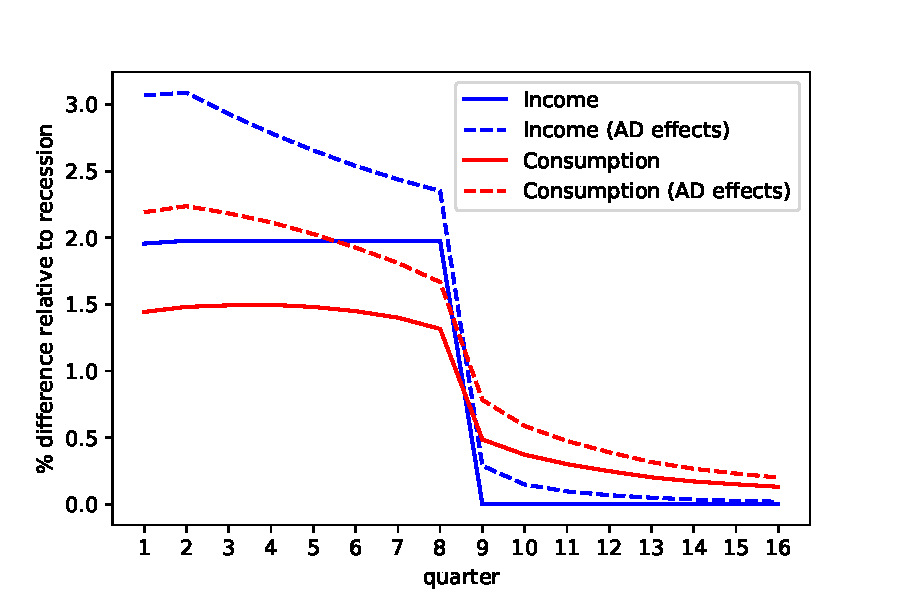
\includegraphics[width=1.2\linewidth]{Code/HA-Models/FromPandemicCode/Figures/recession_taxcut_relrecession}
              \end{column}
            \end{columns}

          \end{frame}
        }{}



        \ifbool{fullcon}{
            
            
            
            


            \begin{frame}
              
              \frametitle{IRFs for stimulus check}
              
              \begin{columns}	
                
                \begin{column}{0.33\textwidth} 	
                  \begin{itemize}[<+->]
                  \item Simulate check policy in recessions lasting  from 1 to 20 q
                  \item Construct probability-weighted sum across rec. lengths
                  \end{itemize}
                \end{column}	
                
                
                \begin{column}{0.66\textwidth}  
                  \centering
                  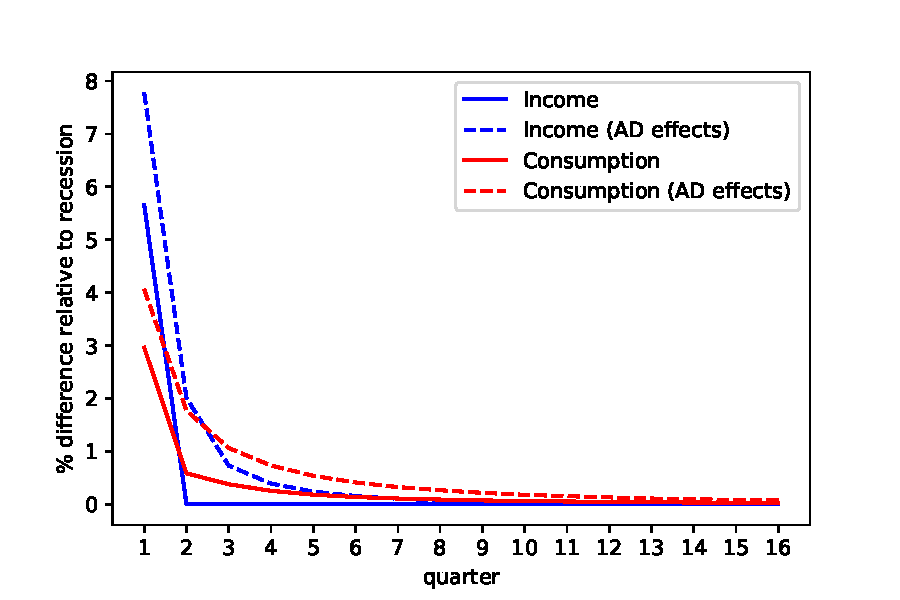
\includegraphics[width=\linewidth]{\econtexRoot/Code/HA-Models/FromPandemicCode/Figures/recession_Check_relrecession}
                \end{column}  
                
              \end{columns}

            \end{frame}

            \begin{frame}
              \frametitle{IRfs for extension of unemployment benefits / payroll tax cut}

              \begin{columns}	
                
                \begin{column}{0.50\textwidth}  	
                  Extension of UI benefits:
                  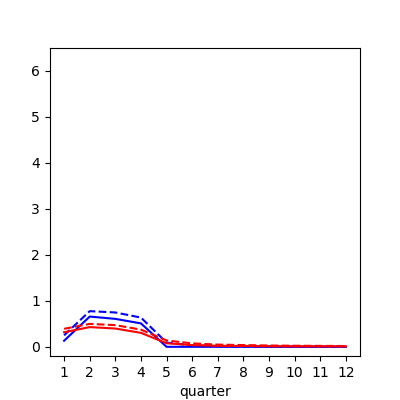
\includegraphics[width=1.2\linewidth]{Code/HA-Models/FromPandemicCode/Figures/recession_UI_relrecession} 
                \end{column}
                
                \begin{column}{0.50\textwidth}  
                  Payroll tax cut:	
                  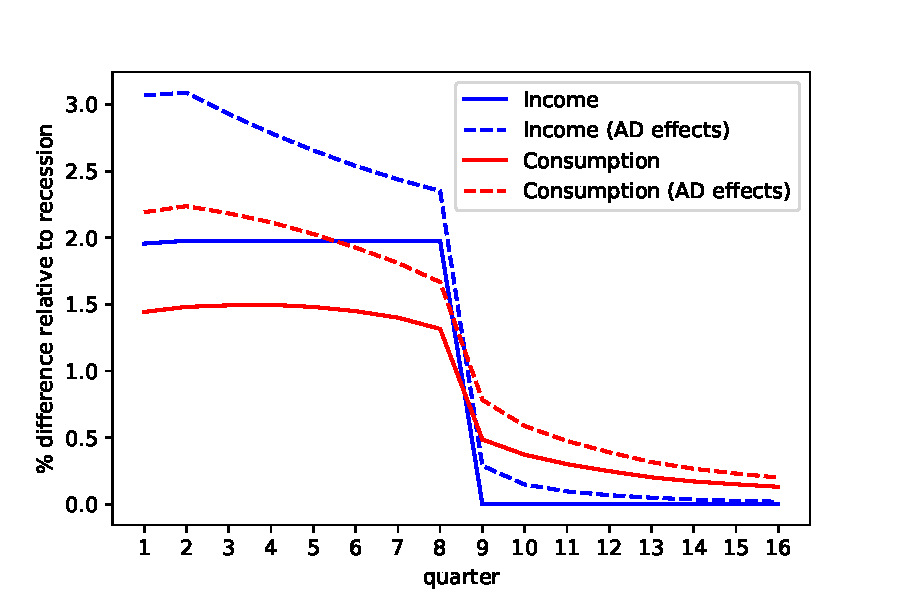
\includegraphics[width=1.2\linewidth]{Code/HA-Models/FromPandemicCode/Figures/recession_taxcut_relrecession}
                \end{column}
              \end{columns}
              
            \end{frame}
            


          }{}




          \begin{frame}
            \frametitle{Multipliers}

            \begin{columns}

              \begin{column}{0.50\textwidth}
                \begin{equation*}
                  M^P_t = \frac{\text{NPV of induced consumption up to $t$}}{\text{NPV of the cost of the policy}}
                \end{equation*}
              \end{column}

              \begin{column}{0.50\textwidth}

                \begin{figure}[t]
                  \centering
                  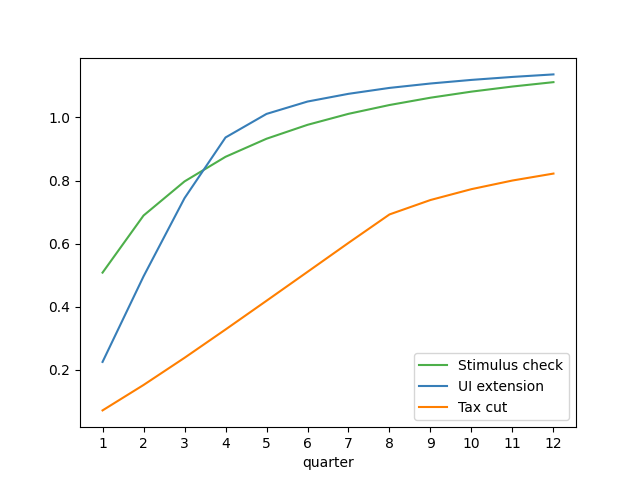
\includegraphics[width=\linewidth]{Code/HA-Models/FromPandemicCode/Figures/Cummulative_multipliers}
                \end{figure}

              \end{column}
            \end{columns}




            \begin{table}[t]
              \center
              \begin{tabular}{@{}lccc@{}} 
                \toprule 
                & Stimulus check    & UI extension    & Tax cut     \\  \midrule 
                10y-horizon Multiplier (no AD effect) &0.872  & 0.910  & 0.847     \\ 
                10y-horizon Multiplier (AD effect) &1.245  & 1.200  & 0.999     \\ 
                % 10y-horizon (1st round AD effect only) &1.162  & 1.140  & 0.967     \\ 
	Share of policy expenditure during recession &100.0\%  & 80.6\%  & 57.6 \%    \\ 
\end{tabular}  
\end{table}

\end{frame}

\begin{frame}
\frametitle{Robustness: Multipliers in HANK}


\begin{figure}
\begin{minipage}[c]{0.48\linewidth}
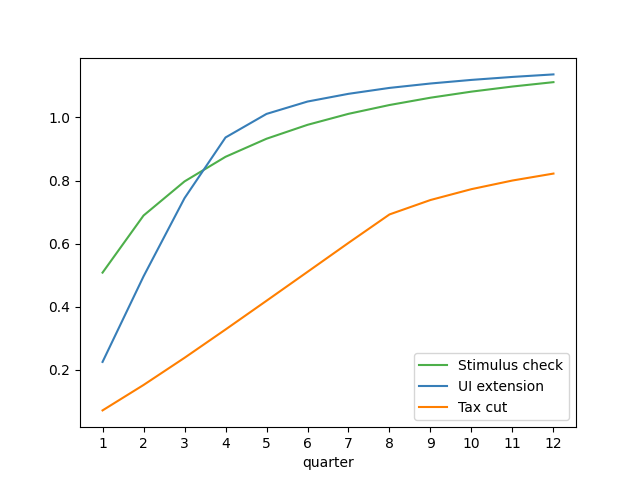
\includegraphics[scale=0.5]{Code/HA-Models/FromPandemicCode/Figures/Cummulative_multipliers}
\vspace{0.2cm}
\captionof{figure}{HA + AD effects}
\end{minipage}
\hfill
\begin{minipage}[c]{0.48\linewidth}
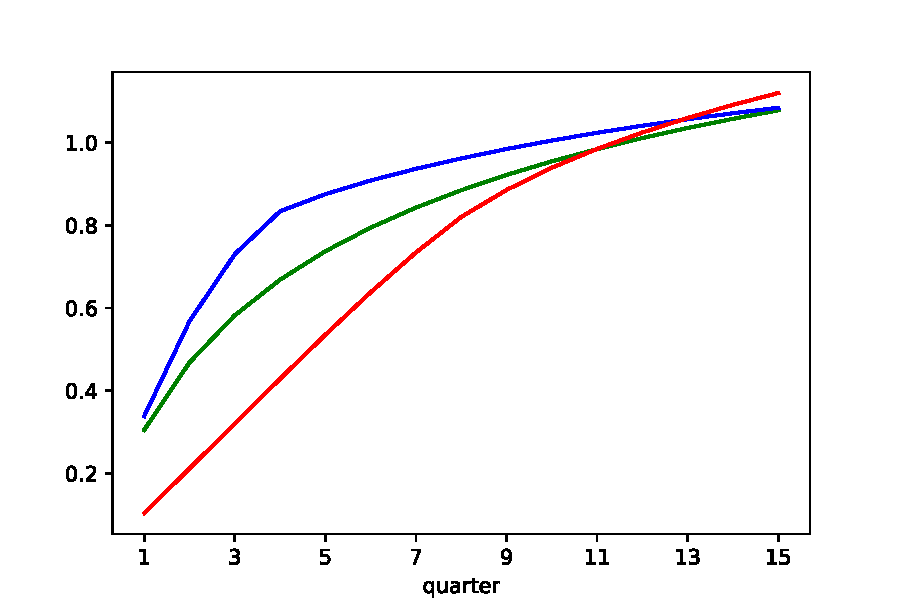
\includegraphics[scale= 0.5]{Code/HA-Models/FromPandemicCode/Figures/Cumulative_multipliers_HANK}
\vspace{0.2cm}
\captionof{figure}{HANK}
\end{minipage}
\end{figure}


\end{frame}


	\begin{frame}
		\frametitle{Welfare measure construction}
		\hypertarget{WelfareMeasure}{}
		
		Guiding principles
		
		\begin{enumerate}
			\item Each consumer is valued equally by the social planner 
			\item Utility from splurge in the same way as other spending
			\item No social benefit to the policies outside of a recession
		\end{enumerate} 
		
		\vspace{0.6cm}
		
		Simple aggregation of consumer util.
only satisfies principle 1 \& 2:
		\begin{equation}\begin{gathered}\begin{aligned}
			\mathcal{W}(\text{policy},Rec,AD) =\frac{1}{N}\sum_{i=1}^{N} \sum_{t=0}^{\infty} \beta_S^t u(\mathbf{c}_{it,\text{policy},Rec,AD})
		\end{aligned}\end{gathered}\end{equation}
		
		\pause
		
		To satisfy principle 3, we calculate
		
		\begin{itemize}[<+->]
			\item Net welfare: Subtract the welfare cost of financing the policy
			\item Recession-based net welfare: Subtract the net welfare impact of policy outside of recession
		\end{itemize}	
	
		\vspace{0.2cm}
		\hyperlink{WelfareMeasure1}{\beamerbutton{Details on welfare measure}}
		
	\end{frame}




\begin{frame}
	\frametitle{Welfare results}
	\centering 
	\begin{tabular}{@{}lccc@{}} 
		\toprule 
		& Check      & UI    & Tax Cut    \\  \midrule 
		Without AD effects & 0.011  & 0.509  & 0.002     \\ 
		With AD effects & 0.151  & 1.101  & 0.056     \\ 
	\end{tabular}  
	\medskip
	\begin{itemize}[<+->]
		\itemsep = .75\bigskipamount 
		\item All policies adjusted to the fiscal size of the UI extension
		\item Interpretation: A welfare gain of x $\Leftrightarrow$ social planner is indifferent between 
		\begin{itemize}[<+->]
			\itemsep = .25\bigskipamount 
			\item the stimulus policy being implemented in response to a recession and 
			\item a permanent increase in the baseline consumption of the total population by x basis points (0.01\% of baseline cons.)
		\end{itemize}
		\item All policies much more effective when mulitplier present
	\end{itemize}
\end{frame}

\begin{frame}
	\frametitle{Conclusion: Comparing the policies}
	\begin{itemize}[<+->]
		\itemsep = .5\bigskipamount 
		\item Comparison of three consumption stimulus policies in a HA model consistent with data on the distribution of liquid wealth and intertemporal MPCs 
		\item Welfare measure: UI extension is the clear bang-for-the-buck winner 
		\item The stimulus check is less well targeted, but\ldots 
		\begin{itemize}[<+->]
			\itemsep = .25\bigskipamount 
			\item is transferred immediately ensuring that money arrives when it is most valuable 
			\item is more easily scaled up to provide more stimulus 
		\end{itemize}
		\item The tax cut is both poorly targeted and may yield substantial spending after the recession is over 
		\item Framework can be used to evaluate other candidate policies 
		
	\end{itemize}
	
\end{frame}



\begin{frame}
	\frametitle{Thank you for your attention!}
	\begin{itemize}[<+->] 
		\item Access the paper, presentation slides and code at: \href{https://github.com/llorracc/HAFiscal}{https://github.com/llorracc/HAFiscal}
	\end{itemize}	

		\begin{figure}
			\centering
			
\includegraphics[width=0.3\linewidth]{"Presentations/QRCode.png"}
		\end{figure}
	
\end{frame}






\section{Appendix}


\begin{frame}
	\frametitle{Parameters describing the policies}
	\label{sli:policies}
	\centering 
	\begin{tabular}{lc}
		\toprule 
		\multicolumn{2}{l}{Parameters describing policy experiments} \\ \midrule 
		Parameter & Value \\ \midrule 
		Change in unemployment rates in a recession & $\times 2$ \\ 
		Expected unemployment spell in a recession & 4 quarters \\ 
		Average length of recession & 6 quarters \\ 
		Size of stimulus check & \$1,200 \\ 
		PI threshold for reducing check size & \$100,000 \\ 
		PI threshold for not receiving check & \$150,000 \\ 
		Extended unemployment benefits & 4 quarters \\
		Length of payroll tax cut & 8 quarters \\ 
		Income increase from payroll tax cut & 2 percent \\ 
		Belief (probability) that tax cut is extended & 50 percent 		
		\\ \bottomrule
	\end{tabular}

	\vspace{1cm}
	\hyperlink{Parameters}{\beamerbutton{Go back}} 
\end{frame}


\begin{frame}
	\frametitle{Welfare measure construction}
	
	Guiding principles
	
	\begin{enumerate}
		\item Each consumer is valued equally by the social planner 
		\item Utility from splurge in the same way as other spending
		\item No social benefit to the policies outside of a recession
	\end{enumerate} 
	
	\vspace{0.6cm}
	\pause
	
	Simple aggregation of consumer util.
only satisfies principle 1 \& 2:
	\begin{equation}\begin{gathered}\begin{aligned}
		\mathcal{W}(\text{policy},Rec,AD) =\frac{1}{N}\sum_{i=1}^{N} \sum_{t=0}^{\infty} \beta_S^t u(\mathbf{c}_{it,\text{policy},Rec,AD}) 
	\end{aligned}\end{gathered}\end{equation}
	
	\begin{itemize}[<+->]
		\item $\mathbf{c}_{it,\text{policy},Rec,AD}$: consumption paths (including splurge) for each consumer / policy
		\item $Rec\in\{1,0\}$: recession indicator, $AD\in\{1,0\}$: AD ind.
		\item $\beta_S = 1/R$: social planner's discount factor 
	\end{itemize}	
	
\end{frame}


\begin{frame}
	\frametitle{Welfare measure construction II}
	\hypertarget{WelfareMeasure1}{}
	
	
	To satisfy principle 3 we define $\mathcal{C}(\text{policy},Rec,AD) =$
	\begin{equation}\begin{gathered}\begin{aligned}
		& \bigg( \underbrace{\frac{\mathcal{W}(\text{policy},Rec,AD)-\mathcal{W}(\text{None},Rec,AD)}{\mathcal{W}^c}}_\text{\RNum{1}}  - \underbrace{\frac{PV(\text{policy},Rec)}{\mathcal{P}^c} }_\text{\RNum{2}} \bigg) \nonumber \\  
		& -
		\bigg( \underbrace{\frac{\mathcal{W}(\text{policy},0,0) - \mathcal{W}(\text{None},0,0)}{\mathcal{W}^c}}_\text{\RNum{3}}  - \underbrace{\frac{PV(\text{policy},0)}{\mathcal{P}^c}}_\text{\RNum{4}}  \bigg) 
	\end{aligned}\end{gathered}\end{equation}
	
	\begin{itemize}[<+->]
		\item \RNum{1}: Policy-induced increase in agg. welfare (in bp of SS-cons.)
		\item \RNum{2}: Cost of policy $\Leftrightarrow$ \RNum{1} - \RNum{2}: Net agg. welfare increase
		\item \RNum{3} - \RNum{4}: Net welfare impact of policy outside of recession
		\item $\mathcal{C}$ measures only welfare effects beyond pure redistribution
	\end{itemize}
	
\end{frame}
	



\begin{frame}
	\frametitle{Robustness: Different replacement rates}
	\centering  
	\small 
	
	\begin{itemize}[<+->]
		\item Discount factor distributions: 
	\end{itemize}

	\begin{table}
		\begin{tabular}{llc|cccccc} 
			\toprule
			& & & \multicolumn{2}{c}{Dropout} & \multicolumn{2}{c}{Highschool} & \multicolumn{2}{c}{College} \\ \midrule 
			& & Splurge & $\beta$ & $\nabla$ & $\beta$ & $\nabla$ & $\beta$ & $\nabla$ \\ \midrule 
			Baseline & ($\rho_{b}=0.7$, $\rho_{nb}=0.5$) & 0.306 & 0.735 & 0.298 & 0.924 & $0.137^{*}$ & 0.984 & 0.010 \\ 
			Altern. & ($\rho_{b}=0.3$,  $\rho_{nb}=0.15$) & 0.306 & 0.609 & $0.445^{*}$ & 0.890 & 0.116 & 0.978 & 0.016
			\\ \bottomrule 
		\end{tabular}
	
	
	\begin{itemize}[<+->]
		\item Welfare results: 
	\end{itemize}
		
		\begin{tabular}{@{}lllll@{}}
			\toprule
			&                    & Stimulus check & UI extension & Tax cut \\ \cmidrule(l){1-5} 
			\multirow{2}{*}{no AD effects} 	& Baseline  ($\rho_{b}=0.7$, $\rho_{nb}=0.5$) 		& 0.011          & 0.509        & 0.002   \\
			& Altern.  ($\rho_{b}=0.3$, $\rho_{nb}=0.15$) 	& 0.043          & 1.845        & 0.003   \\ \cmidrule(l){1-5} 
			\multirow{2}{*}{AD effects}		& Baseline  ($\rho_{b}=0.7$, $\rho_{nb}=0.5$)    	& 0.151          & 1.101        & 0.056   \\
			& Altern.  ($\rho_{b}=0.3$, $\rho_{nb}=0.15$)    & 0.157          & 2.514        & 0.048   \\ \cmidrule(l){1-5} 
		\end{tabular}
	\end{table}
\end{frame}

\begin{frame}
	\frametitle{Robustness: Different interest rates}
	\begin{tabular}{lc|cccccc} 
		\toprule
		& & \multicolumn{2}{c}{Dropout} & \multicolumn{2}{c}{Highschool} & \multicolumn{2}{c}{College} \\ \midrule 
		& Splurge & $\beta$ & $\nabla$ & $\beta$ & $\nabla$ & $\beta$ & $\nabla$ \\ \midrule 
		$R = 1.005$ & 0.307 & 0.740 & 0.298 & 0.927 & $0.193^{*}$ & 0.989 & 0.0082 \\
		$R = 1.01$ (baseline) & 0.307 & 0.735 & 0.298 & 0.924 & $0.137^{*}$ & 0.984 & 0.0096 \\ 
		$R = 1.015$ & 0.307 & 0.724 & $0.357^{*}$ & 0.919 & $0.138^{*}$ & 0.979 & 0.0105 
		\\ \bottomrule 
	\end{tabular}
\end{frame}

\begin{frame}
\frametitle{Robustness: Multipliers in HANK}

\begin{figure}
\begin{minipage}[c]{0.48\linewidth}
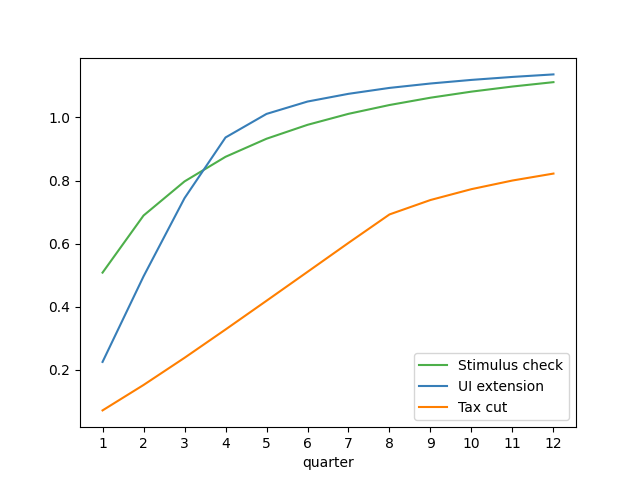
\includegraphics[scale=0.5]{Code/HA-Models/FromPandemicCode/Figures/Cummulative_multipliers}
\vspace{0.2cm}
\captionof{figure}{HA + AD effects}
\end{minipage}
\hfill
\begin{minipage}[c]{0.48\linewidth}
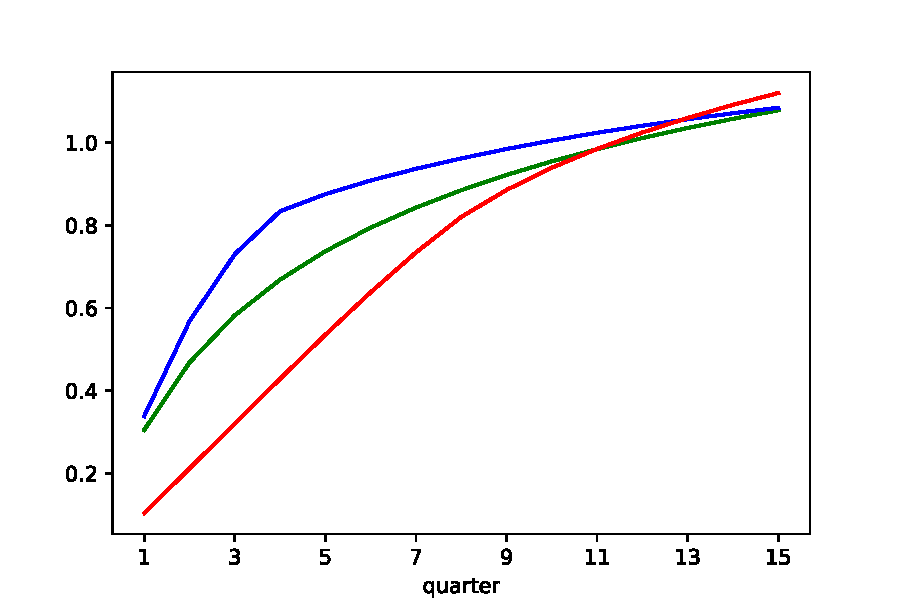
\includegraphics[scale= 0.5]{Code/HA-Models/FromPandemicCode/Figures/Cumulative_multipliers_HANK}
\vspace{0.2cm}
\captionof{figure}{HANK}
\end{minipage}
\end{figure}

\end{frame}
\end{document}
